\section{Methods}\label{sec:method}

\subsection{Normalization of \ac{dce}-\ac{mri} images}\label{sec:norm}

\begin{figure}
  \centering
  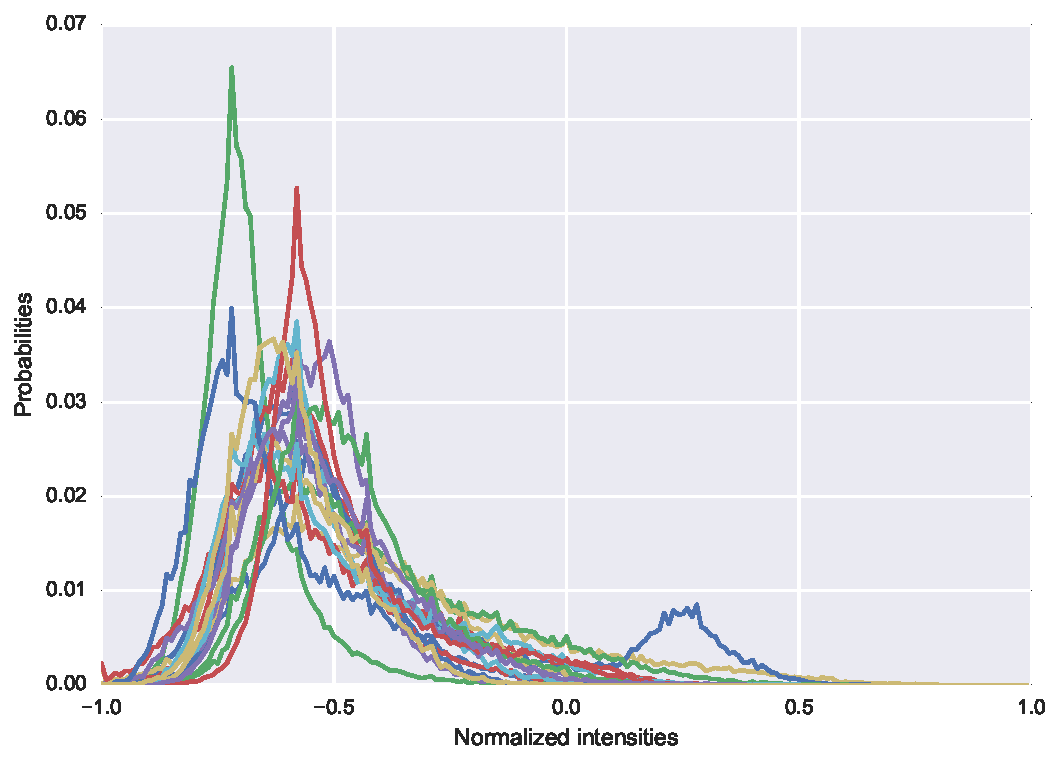
\includegraphics[width=0.7\linewidth]{02_methods/figures/t2w.pdf}
  \caption{Illustration of the inter-patient variations in 17 different patients, using the \acs*{pdf} representation.}
  \label{fig:t2w}
\end{figure}

In this work, we propose a method to normalize \ac{dce}-\ac{mri} prostate data to reduce inter-patient variations, although it can be applied to any \ac{dce}-\ac{mri} sequences.
In \ac{t2w}-\ac{mri}, these variations are characterized by a shift and a scaling of the intensities as illustrated by the intensity \ac{pdf} in Fig.\,\ref{fig:t2w}.
Therefore, these variations can be corrected using a $z$-score approach, assuming that the data follow a specific distribution~\citep{lemaitre2016normalization}.

\begin{figure*}
  \centering
  \hspace*{\fill}
  \subfigure[]{\label{subfig:pathhist}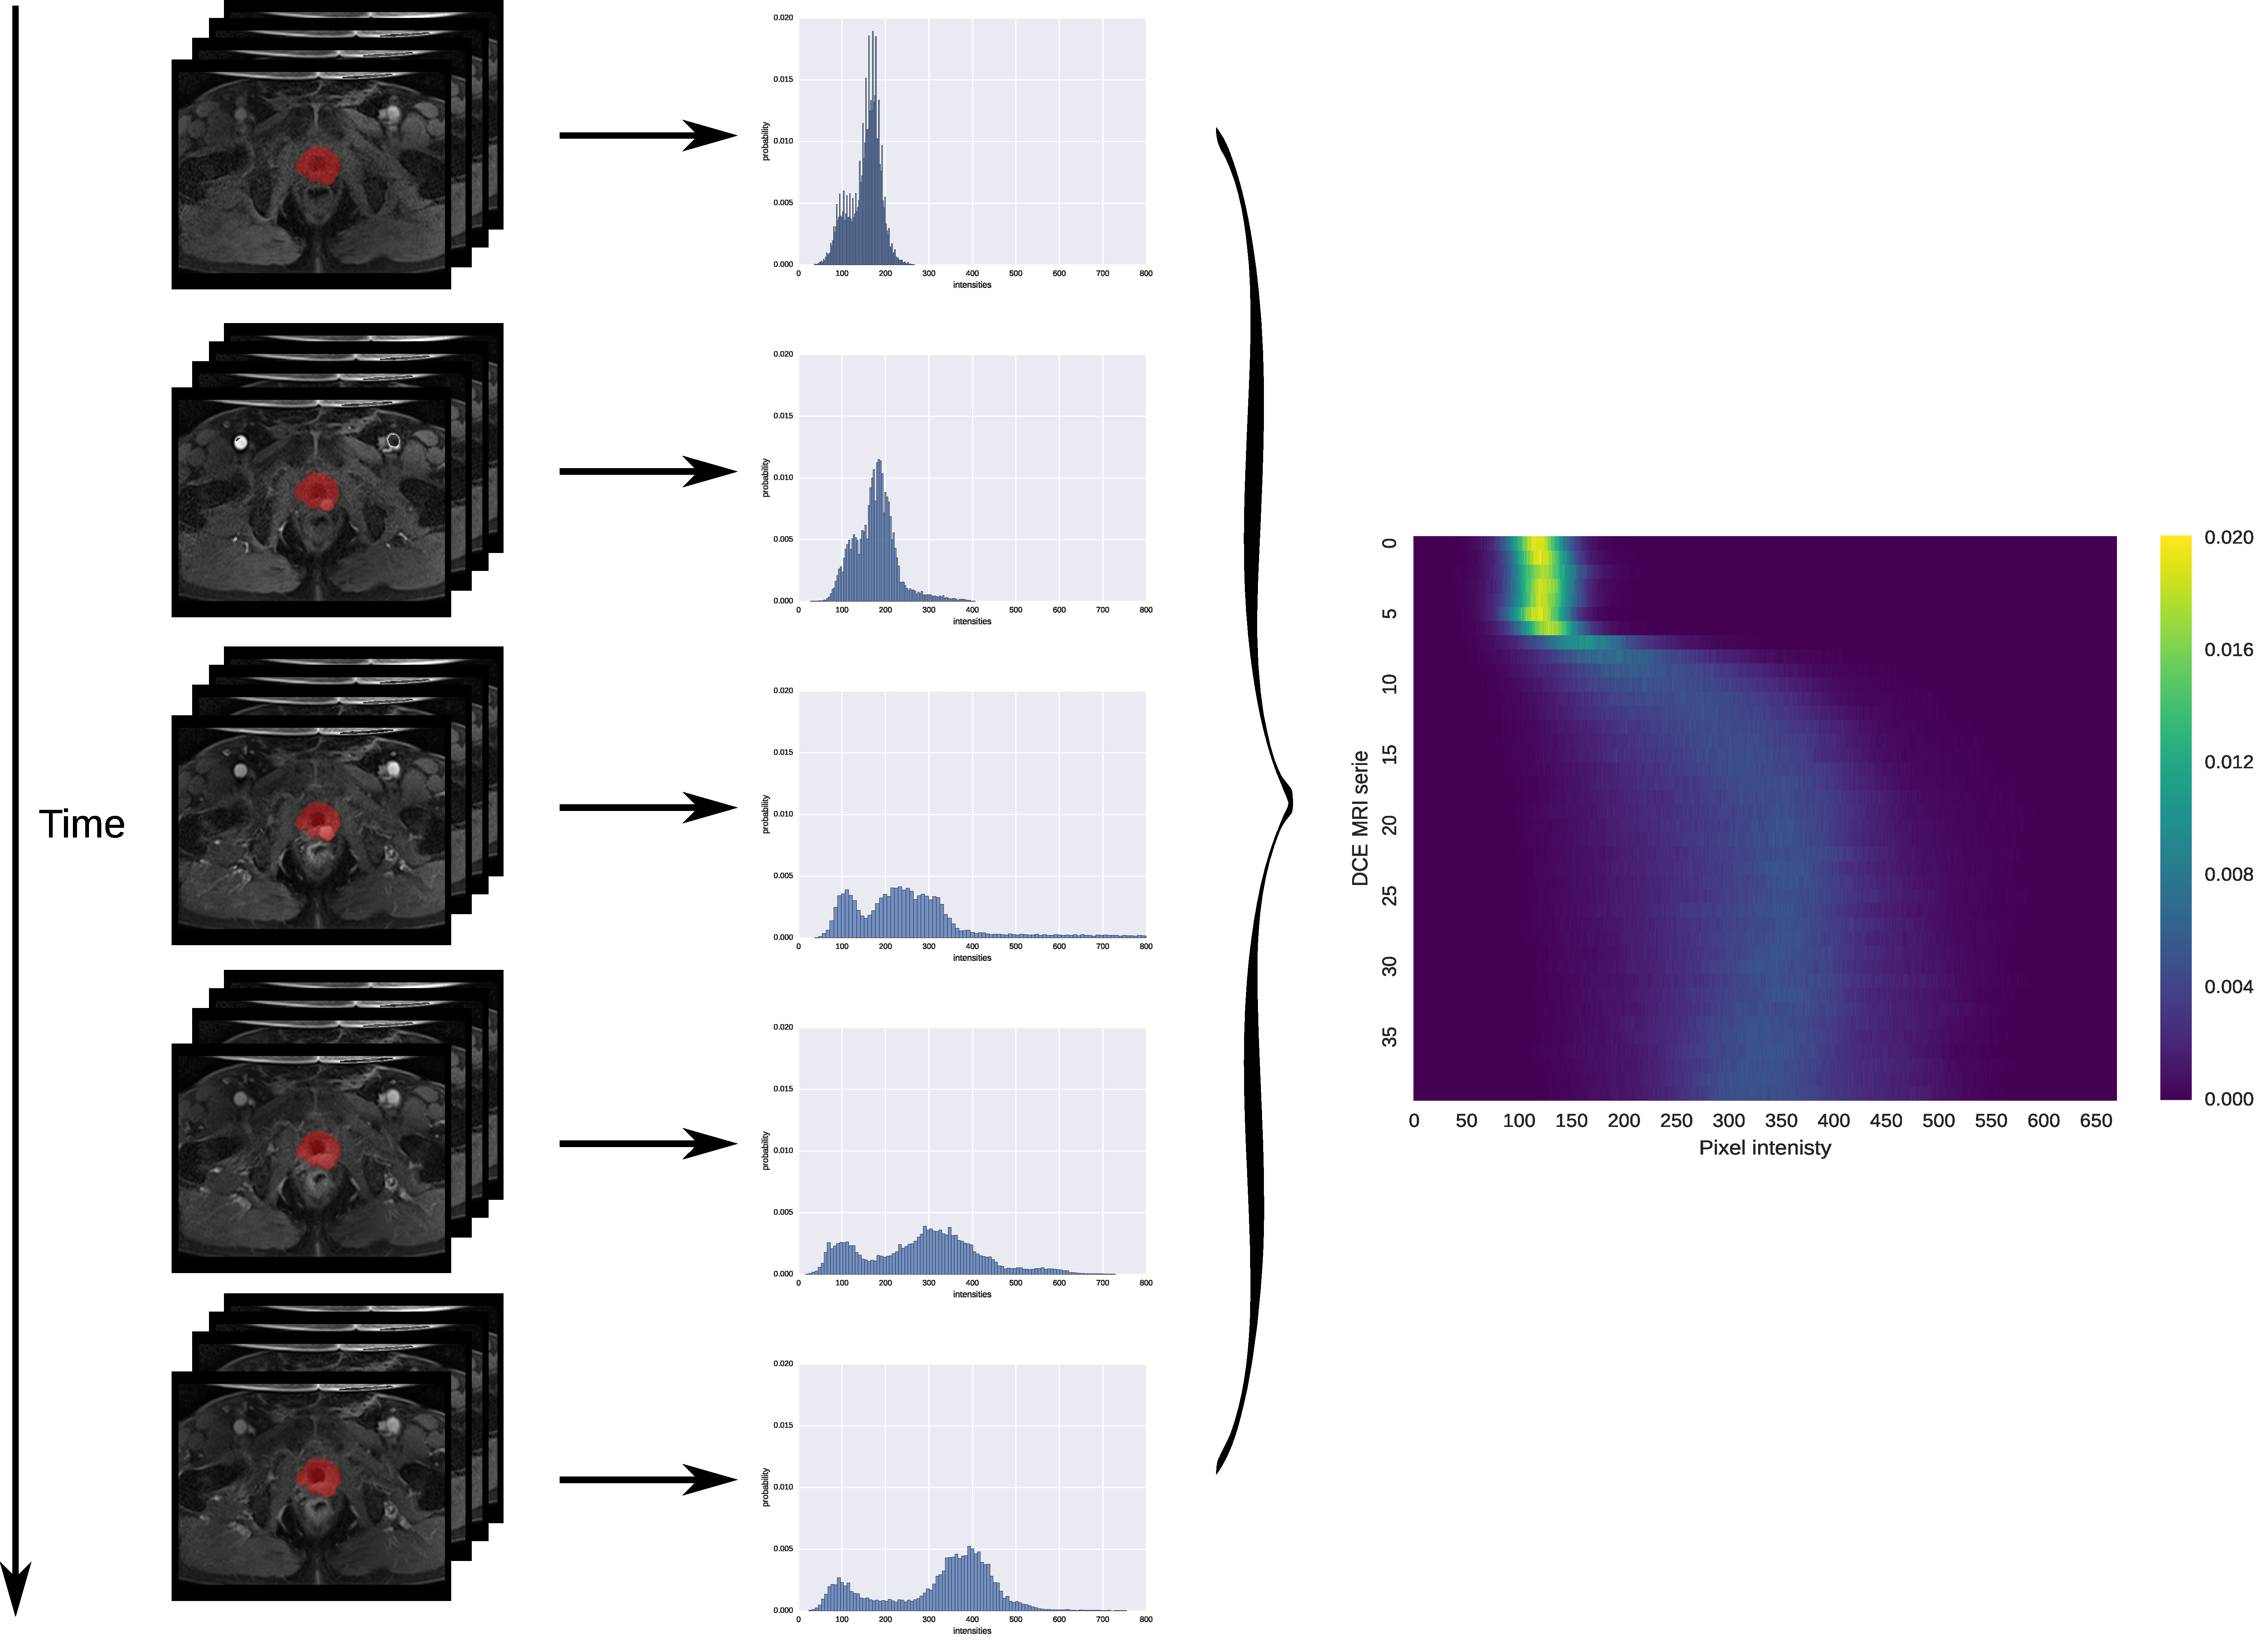
\includegraphics[width=1\textwidth]{02_methods/figures/heatmaprep.pdf}} \hfill
  \hspace*{\fill}
  \\
  \hspace*{\fill}
  \subfigure[]{\label{subfig:pat1}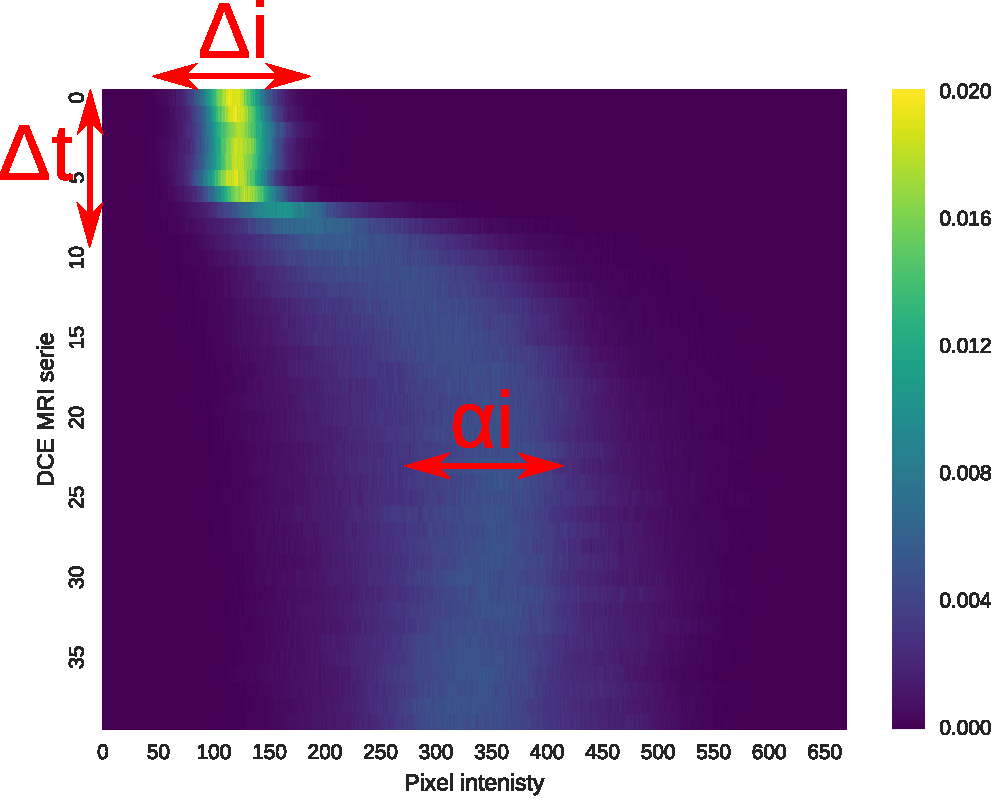
\includegraphics[width=.49\textwidth]{02_methods/figures/pat1_annotated.pdf}} \hfill
  \subfigure[]{\label{subfig:pat2}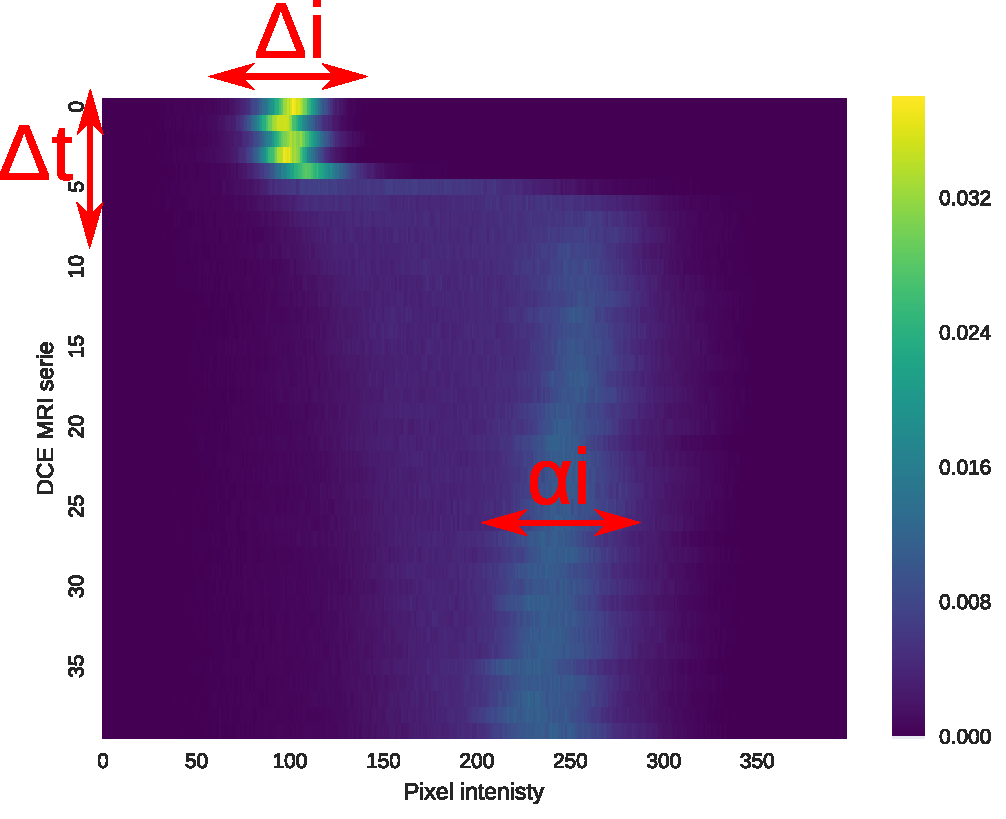
\includegraphics[width=.49\textwidth]{02_methods/figures/pat2_annotated.pdf}} \hfill
  \hspace*{\fill}
  \caption{\subref{subfig:pathhist} Illustration of the heatmap representation: all \ac*{pdf}s of the prostate gland are concatenated together to build an heatmap; \subref{subfig:pat1}-\subref{subfig:pat2} Illustration of inter-patient variations (i.e., $\Delta_i$, $\Delta_t$, and $\alpha_i$) \acs*{pdf} over time of two patients in a \ac{dce}-\ac{mri}.}
  \label{fig:heatmap}
\end{figure*}

In \ac{dce}-\ac{mri}, the intensity \ac{pdf} of prostate gland does not follow a unique type of distribution such as Rician or Gaussian distribution, as shown in Fig.\,\ref{subfig:pathhist}.
Indeed, the inter-patient variations are more complex due to the temporal acquisition.
A better representation to observe these variations is to represent the intensity \ac{pdf} of the prostate gland over time--- requiring to segment the prostate ---using a heatmap representation as shown in Fig.\,\ref{subfig:pathhist}.
Analyzing this heatmap representation across patients (see Fig.\,\ref{subfig:pat2}), the following variations are highlighted:
(i) an intensity offset $\Delta_i$ of the \ac{pdf} peak at pre-contrast,
(ii) a time offset $\Delta_t$ depending of the contrast agent arrival, and
(iii) a change of scale $\alpha_i$ related to the signal enhancement.
Therefore, our normalization method should attenuate all these variations and be performed globally across the different time sequence rather than for each independent sequence.

\subsubsection{Graph-based intensity offsets correction}\label{sec:intoffsets}

\begin{figure}
  \centering
  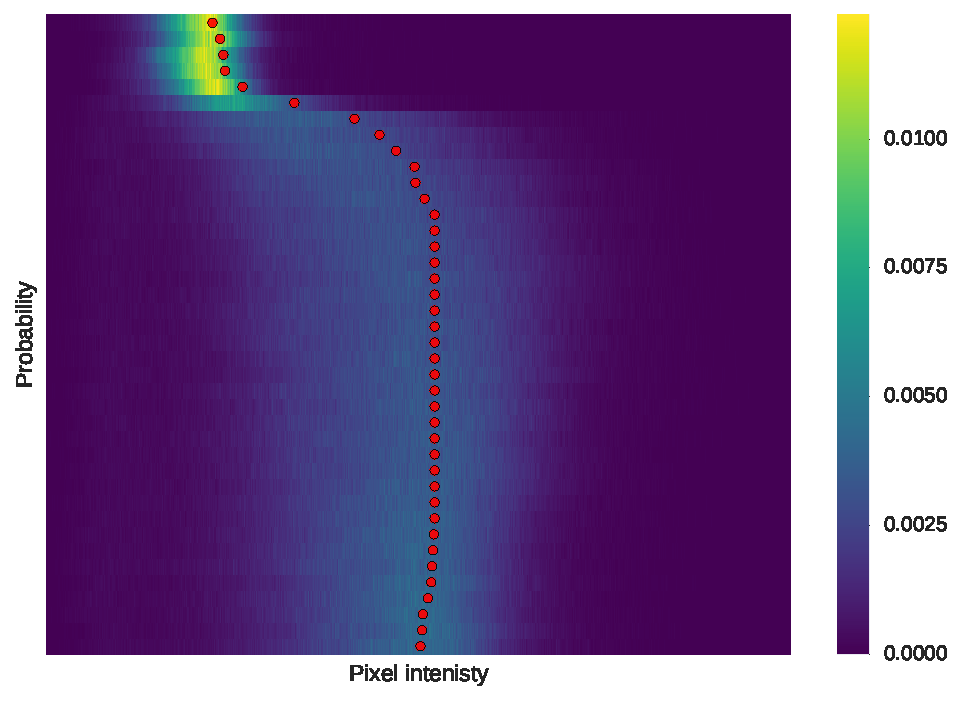
\includegraphics[width=0.7\linewidth]{02_methods/figures/estimator.pdf}
  \caption{Illustration of the estimator found using the shortest-path through the graph.}
  \label{fig:estimator}
\end{figure}

Before to standardize each sequence, the first step of the normalization is to cancel the intensity specific at each patient, occurring due to the media injection.
As previously mentioned, the intensity \ac{pdf} does not always follow either a Rician or a Gaussian distribution over time, in \ac{dce}-\ac{mri}.
Therefore, the mean of these distributions cannot be used as a potential estimate for these offsets.
Additionally, these offsets should be characterized by a smooth transition between series over time.
Thus, this problem is solved using the graph-theory: considering the intensity \ac{pdf} over time as shown in Fig.\,\ref{subfig:pathhist}, the offsets correspond to the boundary splitting the heatmap in two partitions such that they are as close as possible to the peak of the intensity \ac{pdf} (see Fig.\,\ref{fig:estimator} for an illustration).
Given the heatmap, a directed weighted graph $\mathcal{G}=(\mathcal{V}, \mathcal{E})$ is built by taking each bar--- i.e., the probability for a given time and pixel intensity---of the heatmap as a node and connecting each pair of bars by an edge.
The edge weight $w_{ij}$ between two nodes $i$ and $j$ corresponding to two pixels at position $(x_i, y_i)$ and $(x_j, y_j)$, respectively, is defined as in Eq.\,\eqref{eq:weight}:

\begin{equation}
  w_{ij} = \begin{cases}
    \alpha \exp(1 - \frac{H(i)}{\max(H)})       & \text{if } x_j = x_i + 1 \text{ and } y_j = y_i, \\
    (1 - \alpha) \exp(1 - \frac{H(i)}{\max(H)}) & \text{if } x_j = x_i \text{ and } y_j = y_i + 1, \\
    0                                           & \text{otherwise},
  \end{cases}
  \label{eq:weight}
\end{equation}

\noindent where $H$ is the heatmap, $\alpha$ is a smoothing parameter controlling the partitioning.

Therefore, these offsets are estimated by finding the shortest-path to cross the graph using Dijkstra's algorithm.
The entry and exiting nodes are set to be the bin with the maximum probability for the first \ac{dce}-\ac{mri} serie and the bin corresponding to the median value for the last \ac{dce}-\ac{mri} serie, respectively.
To ensure a robust estimation of these offsets, the process of finding the shortest-path is iteratively repeated by shifting the data and updating the heatmap as well as the graph $\mathcal{G}$.
The procedure is stopped once that the offset found does not change.
In general, this process is not repeated more than 3 iterations.
The parameter $\alpha$ is set to $0.9$, empirically.
Figure~\ref{fig:estimator} illustrates the final estimation of the offsets (i.e., red landmark) found for each \ac{dce}-\ac{mri} serie.
Therefore, each intensity offset is subtracted for each \ac{dce}-\ac{mri}.

\subsubsection{Time offset and data dispersion correction}

\begin{figure*}
  \centering
  \hspace*{\fill}
  \subfigure[\acs*{rmse} computed for each patient of our dataset.]{\label{fig:rmse}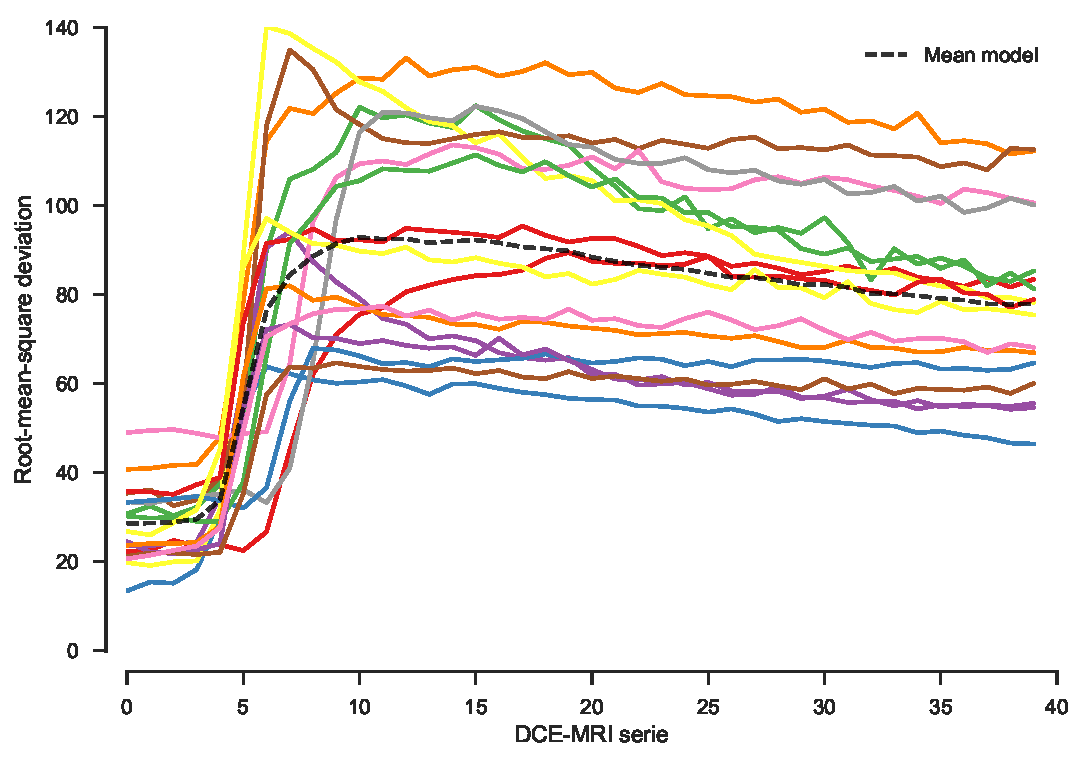
\includegraphics[width=.49\textwidth]{02_methods/figures/rmse.pdf}} \hfill
  \subfigure[\acs*{rmse} after alignment using the curve parametric model.]{\label{fig:rmseal}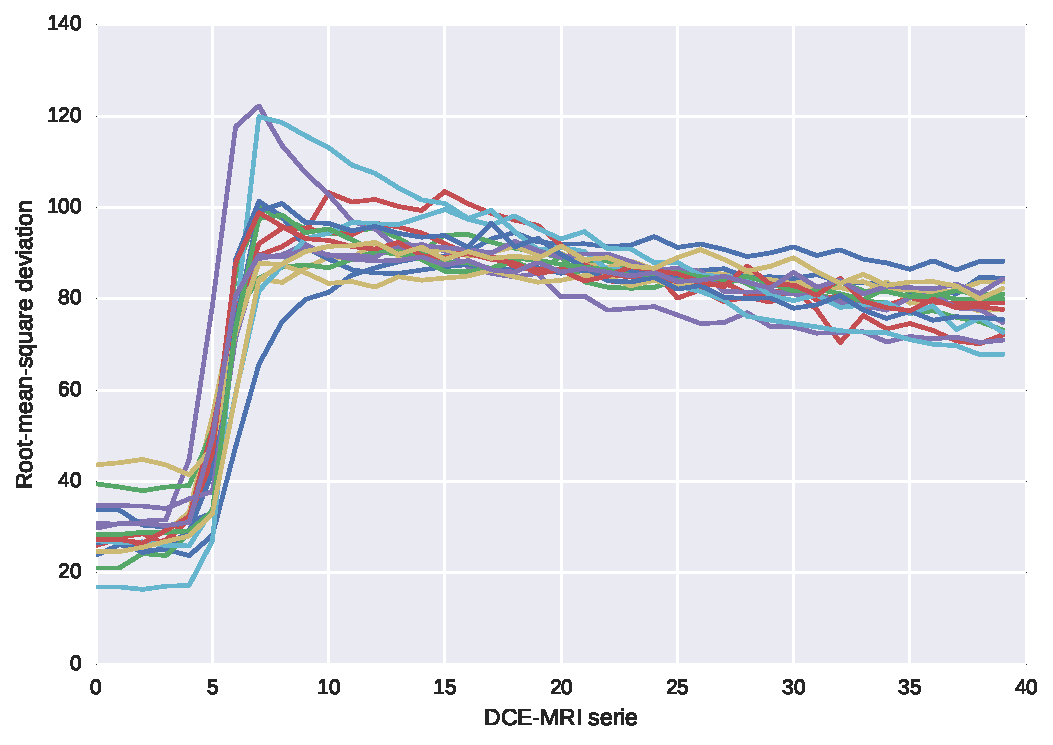
\includegraphics[width=.49\textwidth]{02_methods/figures/rmse_aligned.pdf}}
  \hspace*{\fill}
  \caption{Illustration of the correction of the time offset and the data dispersion.}
  \label{fig:curveal}
\end{figure*}

The next variations to correct are the time offset and the data dispersion.
By computing the \ac{rmse} of the intensities for each \ac{dce}-\ac{mri} serie, one can observe these two variations as shown in Fig.\,\ref{fig:rmse}.
Therefore, to correct these variations, we propose to register each patient \ac{rmse} to a mean model which corresponds to the mean of all patients \ac{rmse}.
The parametric model to perform the registration is formulated as in Eq.\,\eqref{eq:model}:

\begin{equation}
  T(\alpha, \tau, f(t)) = \alpha f(t - \tau) ,
  \label{eq:model}
\end{equation}

\noindent where $\alpha$ and $\tau$ are the two parameters handling the time offset and global scale, respectively, $f(\cdot)$ is the \ac{rmse} function define as:

\begin{equation}
  f(t) = \sqrt{ \left( \frac{\sum_{n=1}^{N} x(t)_{n}^2}{N}  \right) },
  \label{eq:rmsd}
\end{equation}

\noindent where $x(t)_n$ is the shifted intensity of a sample from a specific \ac{dce}-\ac{mri} serie at time $t$ from a total number of $N$ samples.

Therefore the registration problem is equivalent to:

\begin{equation}
  \argmin_{\alpha, \tau} = \sum_{t=1}^{N} \left[ T\left(\alpha, \tau, f(t)\right) - \mu(t) \right]^{2} ,
  \label{eq:cost}
\end{equation}

\noindent where $\mu(\cdot)$ is the mean model, $N$ is the number of \ac{dce}-\ac{mri} serie.

Illustration of the correction applied to each \ac{rmse} patient is shown in Fig.\,\ref{fig:rmseal}.
Once all these parameters have been inferred, the data are shifted as well as scaled.

The resulting normalized data can be classified into two fashions: (i) each normalized signal can be classified considering the whole \ac{dce}-\ac{mri} signal or (ii) the normalized data can be fitted using a quantitative method, as presented in the next section.
However, in the second strategy, this is necessary to apply common intensity offsets such that the data follow a shape as expected by the different quantitative models.
The set of offsets applied is in fact corresponding to the maximum offsets found in Sect.\,\ref{sec:intoffsets}.

\subsection{Quantification of \ac{dce}-\ac{mri}}\label{sec:stateart}

In this section, we summarize the different methods which have been used for the quantification of \ac{dce}-\ac{mri} for \ac{cap} detection~\citep{lemaitre2015computer} and which will be used for comparison in this work.
Furthermore, we would like to emphasize the following additional contributions: (i) a novel automatic \ac{aif} estimation algorithm based on clustering and (ii) a simplified semi-quantitative method using constrained optimization.

\subsubsection{Brix and Hoffmann models}\label{sec:brixhoffmann}

In the Brix model~\citep{brix1991pharmacokinetic}, the \ac{mri} signal intensity is assumed to be proportional to the media concentration.
Therefore, the model is expressed as in Eq.\,\eqref{eq:brix}:

\begin{equation}
  s_n(t) = 1 + A \left[ \frac{\exp(k_{el} t') - 1}{k_{ep}(k_{ep} - k_{el})} \exp(- k_{el} t) - \frac{\exp(k_{ep} t') - 1}{k_{el}(k_{ep} - k_{el})} \exp(- k_{ep} t) \right],
  \label{eq:brix}
\end{equation}

\noindent with

\begin{equation}
  s_n(t) = \frac{s(t)}{S_0},
  \label{eq:enh}
\end{equation}

\noindent where $s(t)$ and $S_0$ are the \ac{mri} signal intensity at time $t$ and the average pre-contrast \ac{mri} signal intensity, respectively; $A$, $k_{el}$, and $k_{ep}$ are the constant proportional to the transfer constant, the diffusion rate constant, and the rate constant, respectively.
Additionally, $t'$ is set such that $0 \leq t \leq \tau$, $t' = t$ and afterwards while $t > \tau$, $t' = \tau$.

\citeauthor{hoffmann1995pharmacokinetic} proposed a similar model as expressed in Eq.\,\eqref{eq:hoffmann}, which derive from the Brix model:

\begin{equation}
  \small
  s_n(t) = 1 + \frac{A}{\tau} \left[ \frac{k_{ep} \left( \exp(k_{el} t') - 1 \right)}{k_{el}(k_{ep} - k_{el})} \exp(- k_{el} t) - \frac{\exp(k_{ep} t') - 1}{(k_{ep} - k_{el})} \exp(- k_{ep} t) \right] ,
  \label{eq:hoffmann}
\end{equation}

\noindent in which the constant $A$ is redefined by isolating the parameter $\tau$.

The parameters $A$, $k_{el}$, and $k_{ep}$ are estimated by fitting the model using non-linear least-squares optimization solved with Levenberg-Marcquardt.

\subsubsection{Tofts model}\label{sec:tofts}

The extended Tofts model is formulated as in Eq.\,\eqref{eq:exttofts}:

\begin{equation}
  C_t(t) = K_{trans} C_p(t) \Conv \exp(-k_{ep}t) + v_p C_p(t),
  \label{eq:exttofts}
\end{equation}

\noindent where $\Conv$ is the convolution operator; $C_t(t)$ and $C_p(t)$ are the concentrations of contrast agent in the tissue and in the plasma, respectively; $K_{trans}$, $k_{ep}$, and $v_p$ are the volume transfer constant, the diffusion rate constant, and the plasma volume fraction, respectively.

Therefore, Tofts model requires to:
(i) detect candidate voxels from the femoral or iliac arteries and estimate a patient-based \ac{aif} signal,
(ii) convert the \ac{mri} signal intensity (i.e., \ac{aif} and dynamic signal) to a concentration, and
(iii) in the case of a population-based \ac{aif}, estimate an \ac{aif} signal.

\begin{figure*}
  \centering
  \hspace*{\fill}
  \subfigure[Original image.]{\label{fig:org}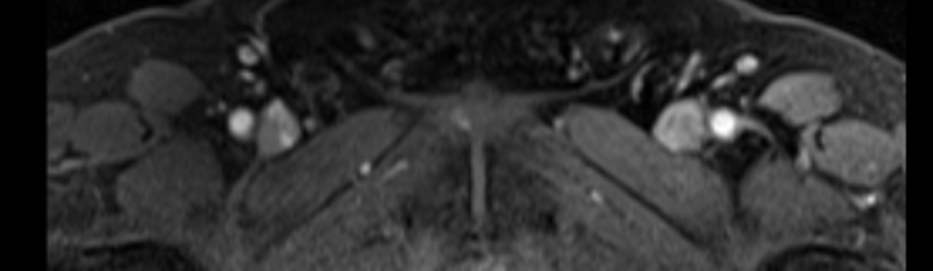
\includegraphics[width=.3\textwidth]{02_methods/figures/original.pdf}} \hfill
  \subfigure[Candidates region after clustering.]{\label{fig:cand}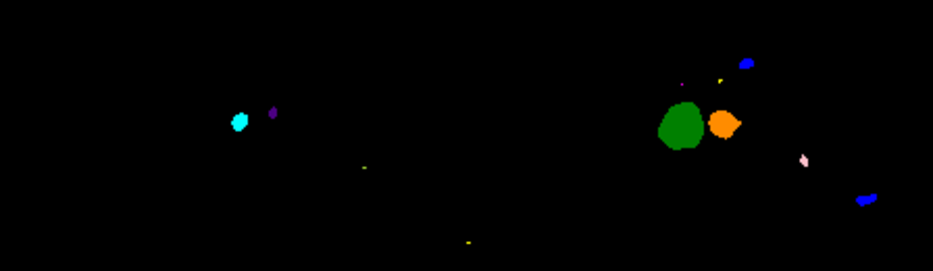
\includegraphics[width=.3\textwidth]{02_methods/figures/candidate.pdf}} \hfill
  \subfigure[Regions selected after applying the different criteria.]{\label{fig:final}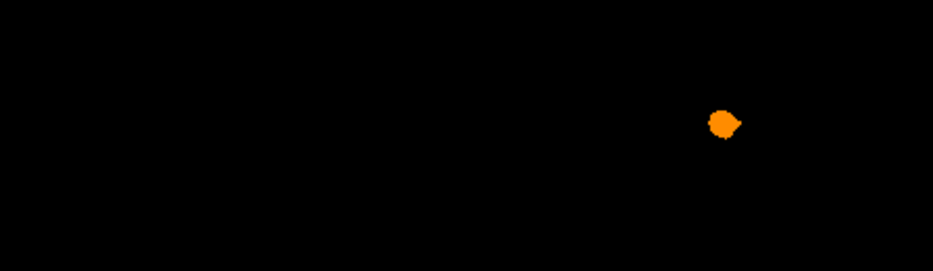
\includegraphics[width=.3\textwidth]{02_methods/figures/aif.pdf}}
  \hspace*{\fill}
  \caption{Illustration of the segmentation of the area used to determine the \acs*{aif}.}
  \label{fig:aif}
\end{figure*}

\begin{description}
  \item[Segmentation of artery voxels and patient-based \ac{aif} estimation] The \ac{aif} signal from \ac{dce}-\ac{mri} can be manually estimated by selecting the most-enhanced voxels from the femoral or iliac arteries~\citep{meng2010comparison}.
    Few methods have been proposed to address the automated extraction of \ac{aif} signal.
    \citeauthor{chen2008automatic} filtered successively the possible candidates to be considered as \ac{aif} such that~\citep{chen2008automatic}:
    (i) dynamic signals with small peak and voxels with a small wash-in are rejected by thresholding,
    (ii) a blob detector is used and large enough regions are kept, and
    (iii) circular and cylindricality criteria are used to reject the last false positive.
    \citeauthor{zhu2011automated} proposed an iterative method selecting voxels which best fit a gamma variate function~\citep{zhu2011automated}.
    However, it requires to compute first and second derivatives as well as maximum curvature points.
    \citeauthor{shanbhag2012generalized} proposed a 4-steps algorithm~\citep{shanbhag2012generalized,fennessy2015quantitative}:
    (i) remove slices with artefacts and find the best slices based on intrinsic anatomic landmarks and enhancement characteristics,
    (ii) find the voxel candidates using the maximum enhanced voxels and a multi-label maximum entropy based thresholding algorithm,
    (iii) exclude region next to the endorectal coil, and
    (iv) select the best 5 candidates which meet enhancement characteristics and that are correlated.

    All the above methods are rather complex and thus we propose a method which is based on the following simple assumptions:
    (i) all possible \ac{aif} signal candidates should have a similar shape,
    (ii) a high enhancement, and
    (iii) the arteries should be almost round and within a size range.
    Therefore, each slice is clustered into regions using K-means clustering with $k=6$.
    The cluster with the highest enhancement\textemdash i.e. corresponding to the 90\textsuperscript{th} percentile of the maximum of each dynamic signal\textemdash contain the arteries and is selected.
    Finally, regions with an eccentricity smaller than $0.5$ and an area in the range of $[100, 400]$ voxels are kept.
    Additionally, to remove voxels contaminated by partial volume effect, only the $10\%$ most enhanced voxels of the possible candidates are kept as proposed by~\citep{schabel2008uncertainty} and the average signal is computed.
    A summary of the different segmentation steps is presented in Fig.\,\ref{fig:aif}.
    \item[Conversion of \ac{mri} signal intensity to concentration] To estimate the free parameters of the Tofts model (see Eq.\,\eqref{eq:exttofts}), the concentration $C_t(t)$ and $C_p(t)$ need to be computed from the \ac{mri} signal intensity and the \ac{aif} signal, respectively.
      This conversion is based on the equation of the FLASH sequence\textemdash see~\ref{app:signaltoconc} for details\textemdash and is formulated as in Eq.\,\eqref{eq:conv}:
      \begin{equation}
        c(t) = \frac{1}{TR \cdot r_1} \ln\left( \frac{1 - \cos \alpha \cdot S^{*}\frac{s(t)}{S_0}}{1 - S^{*}\frac{s(t)}{S_0}} \right) - \frac{R_{10}}{r_1} ,
        \label{eq:conv}
      \end{equation}
      \noindent with,
      \begin{equation}
        S^{*} = \frac{1 - \exp(- TR \cdot R_{10})}{1 - \cos \alpha \cdot \exp(- TR \cdot R_{10})} ,
        \label{eq:sstarconv}
      \end{equation}
      \noindent where $s(t)$ is the \ac{mri} signal, $S_0$ is the \ac{mri} signal prior to the injection of the contrast media, $\alpha$ is the flip angle, $TR$ is the \acf{tr}, $R_{10}$ is the pre-contrast tissue relaxation time also equal to $\frac{1}{T_{10}}$, $r_1$ is the relaxitivity coefficient of the contrast agent.

      $T_{10}$ can be estimated from the acquisition of a T$_1$ map.
      However, this modality is not part of the clinical trial in this research and the value of $T_{10}$ is fixed to \SI{1600}{\ms} for both blood and prostate, in accordance with the values found in the literature~\citep{fennessy2015quantitative,de2004mr,carr2011magnetic}.
      \item[Estimation of population-based \ac{aif}] While estimating the pharmacokinetic parameters from Tofts model, the \ac{aif} concentration $C_p(t)$ can be computed either from the patient or a population.
        We presented in the two previous sections the algorithms which allows to estimate the patient-based \ac{aif} concentration.
        To compare with the previous approach, we also computed a population-based \ac{aif} which will be also used later to compare the performance of both approaches.
        In that regard, the population-based \ac{aif} was estimated as in~\citep{meng2010comparison} by fitting the average patient-based \ac{aif}s to the model of~\cite{parker2006experimentally} which is formulated as in Eq.\,\eqref{eq:parker}:
        \begin{equation}
          C_p(t) = \sum_{n=1}^{2} \frac{A_n}{\sigma_n \sqrt{2 \pi}} \exp\left(\frac{- (t- T_n)^2}{2\sigma_{n}^{2}}\right) + \frac{\alpha \exp(-\beta t)}{1 + \exp{-s (t - \tau)}} ,
          \label{eq:parker}
        \end{equation}
        \noindent where $A_n$, $T_n$, and $\sigma_n$ are the scaling constants, centers, and widths of the n\textsuperscript{th} Gaussian, $\alpha$ and $\beta$ are the amplitude and decay constant of the exponential; and $s$ and $\tau$ are the width and center of the sigmoid function, respectively.
\end{description}

The parameters are estimated by fitting the model using a constrained non-linear least-squares optimization, solved with Trust Region Reflective algorithm~\citep{sorensen1982newton} and bounding the parameters to be positive.

\subsubsection{\acs*{pun} model}\label{sec:pun}

\citeauthor{gliozzi2011phenomenological} showed that \ac{pun} approach can be used for \ac{dce}-\ac{mri} analysis~\citep{gliozzi2011phenomenological}.
The model has been successfully used in a \ac{cad} system proposed by~\cite{giannini2015fully}.
This model can be expressed as in Eq.\,\eqref{eq:pun}:

\begin{equation}
  s_n(t) = \exp\left[rt + \frac{1}{\beta} \left( a_0 - r \right) \left( \exp(\beta t) - 1 \right) \right],
  \label{eq:pun}
\end{equation}

\noindent with

\begin{equation}
  s_n(t) = \frac{s(t) - S_0}{S_0},
  \label{eq:enh}
\end{equation}

\noindent where $s(t)$ and $S_0$ are the \ac{mri} signal intensity at time $t$ and the average pre-contrast \ac{mri} signal intensity, respectively; $r$, $a_0$, and $\beta$ are the free parameters of the model.

The parameters are estimated by fitting the model using non-linear least-squares optimization solved with Levenberg-Marcquardt.

\subsubsection{Semi-quantitative analysis}\label{sec:semi}

The semi-quantitative analysis of the \ac{dce}-\ac{mri} is equivalent to extracting curve characteristics directly from the signal without a strict theoretical pharmacokinetic meaning.
In this work, we use the model presented by~\cite{huisman2001accurate} which formulated the \ac{mri} signal as in Eq.\,\eqref{eq:huisman}:

\begin{equation}
  s(t) = \begin{cases}
    S_0 & 0 \leq t \leq t_0 \\
    S_M - (S_M - S_0) \exp\left( \frac{-(t - t_0)}{\tau} \right) & t_0 < t \leq t_0 + 2 \tau \\
    S_M - (S_M - S_0) \exp\left( \frac{-(t - t_0)}{\tau} \right) + w(t - t_0 + 2 \tau) & t > t_0 + 2 \tau
  \end{cases}
  \label{eq:huisman}
\end{equation}

\noindent where $s(t)$ is the \ac{mri} signal intensity, $S_0$ is the pre-contrast signal intensity, $t_0$ is the time corresponding to the start of enhancement, $S_M$ and $\tau$ is the maximum of the signal and the exponential time constant, and $w$ is the slope of the linear part.

\citeauthor{huisman2001accurate} argue that curve fitting via least-squares minimization using Nelder-Mead algorithm leads to inaccurate estimation of the free parameters: mainly the issue come from an incorrect estimation of the start of enhancement $t_0$ leading to incorrect estimation of the other parameters.
Therefore, they propose to:
(i) estimate robustly $t_0$,
(ii) estimate $S_0$ by averaging the samples between $0$ and $t_0$
(ii) estimate $w$ depending if the slope is significant or not,
(iii) estimate $S_M$ which should be the point at the intersection of the most probable slope line and the plateau.

Instead of these successive estimations, we propose a unified optimization in which $t_0$ is fixed since that this is a key parameter.
Therefore, $t_0$ is robustly estimated from the \ac{aif} signal since that this is the most enhanced signal in which the start of enhancement is easily identifiable.
The \ac{aif} signal is computed as in Section~\ref{sec:tofts}.
$t_0$ is estimated by finding the maximum of the first derivative of the \ac{aif} signal, always occurring at the beginning of the signal.
Then, the function in Eq.\,\eqref{eq:huisman} is fitted using non-linear least squares with Trust Region Reflective algorithm~\citep{sorensen1982newton}.
Furthermore, the parameters $\tau$ and $S_M$ are bounded during the optimization to ensure robust estimations.
$\tau$ is bounded between $t_0$ and $t_f$ which is the time of the last sample while $S_M$ is bounded between $S_0$ and $\max(s(t))$.


From Eq.\,\eqref{eq:huisman}, the following features are extracted:
(i) the wash-in corresponding to the slope between $t_0$ and $t_0 + 2 \tau$,
(ii) the wash-out corresponding to the parameter $w$,
(iii) the area under the curve between $t_0$ and the end of the signal,
(iv) the exponential time constant $\tau$, and
(v) the relative enhancement $S_M - S_0$.

%%% Local Variables: 
%%% mode: latex
%%% TeX-master: "../main"
%%% End: 
